\documentclass[12pt]{amsart}
\pagestyle{plain}

\usepackage{amsthm, setspace, framed, hyperref}
\usepackage[pdftex]{graphicx}
\usepackage{enumerate}

\usepackage[left=1in, right=1in, top=1in, bottom=1in]{geometry}
\setlength\parindent{0pt}

\theoremstyle{plain}
\newtheorem{thm}{Theorem}[section]
\newtheorem{lem}[thm]{Lemma}
\newtheorem*{cor}{Corollary}
\newtheorem{quest}{Question}
\theoremstyle{definition}
\newtheorem*{defn}{Definition}
\newtheorem*{ex}{Example}

\begin{document}
\title[]{Cryptography Mission 02 Solutions}
\begin{tabular*}{\textwidth}{@{\extracolsep{\fill}}l l}
MATH/CSCI 408  & Name: \rule{7cm}{0.5pt} \\
\hline\hline
\end{tabular*} \\
\maketitle

\begin{center}\textbf{Deadline: Thursday, 8 September 2016 at 3:05pm}\\

This mission covers Sections 2.4, 2.6, and 2.7.
\end{center}


\section{Graded Problems}

\begin{enumerate}[1.]
	\item Read the Wikipedia article on the Pigpen cipher:\\ \url{https://en.wikipedia.org/wiki/Pigpen_cipher}.
	\begin{enumerate}[a.]
	\item Replicate the set of all graphical symbols on your homework here:
	\begin{framed}
	\begin{center}
	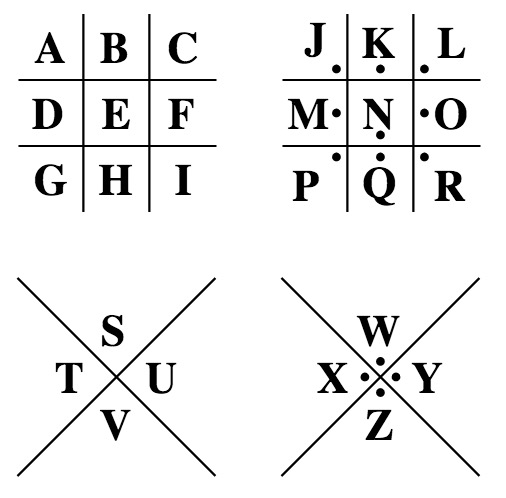
\includegraphics[height=1.5in]{Pigpen.jpg}
	\end{center}
	\end{framed}
	\item Encrypt the message ``you only live twice" using the Pigpen cipher.
	\begin{framed}
	\begin{center}
	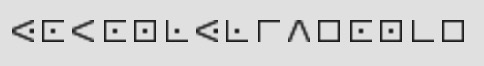
\includegraphics[width=2in]{Pigpen02.jpg}
	(from \url{https://cryptii.com/text/pigpen})
	\end{center}
	\end{framed}
	\end{enumerate}
	\item On Moodle, download and work through the ``Encryption.sagews" code.\\
		\begin{enumerate}[a.]
		\item Using the Caesar cipher with a shift of 12, encrypt ``Julius No".\\
		\begin{framed}
		VGXUGEZA
		\end{framed}
		\item Follow the link mentioned in the SageMath code (recopied here: \url{http://doc.sagemath.org/html/en/reference/cryptography/sage/crypto/classical.html}).  Read through the documentation of the TranspositionCipher.  In a sentence or two, describe what the Transposition Cipher does to a plaintext phrase:
		\begin{framed}
		The Transposition Cipher changes the orders of the letters in a plaintext phrase.  In the example, it reverses the order of the letters.
		\end{framed}
		\item Use some SageMath code and the Transposition Cipher to encrypt: ``\texttt{BABOUTHEOCELOT}" (note that normally, we use lowercase for plaintext, but we need all caps for this particular line of code).
		\begin{framed}
		\begin{center}
		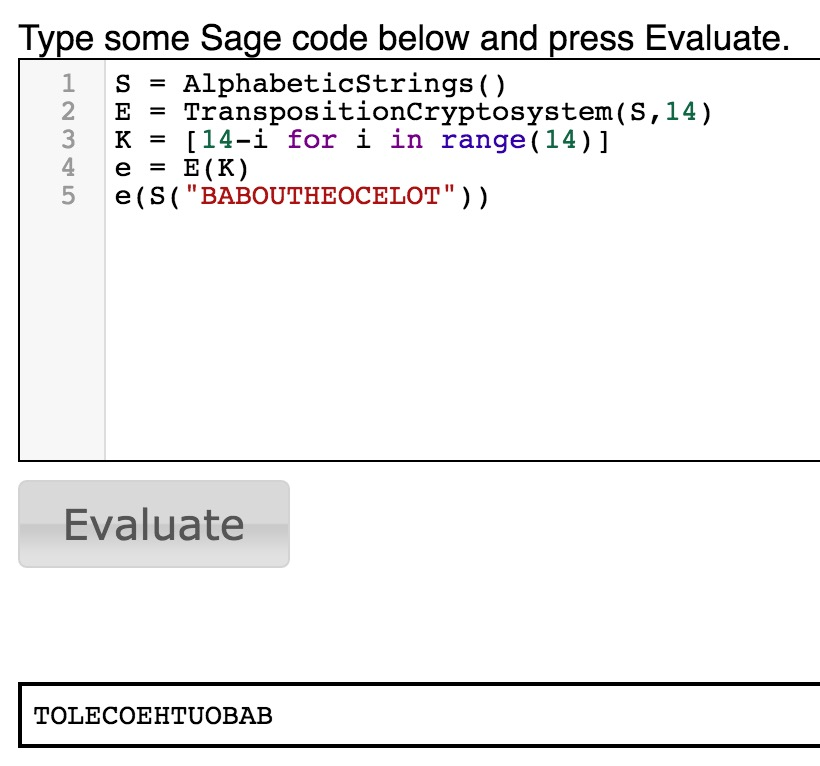
\includegraphics[height=3in]{Transposition.jpg}
		\end{center}
		\end{framed}
		\end{enumerate}
	\item (T \& W 2.13 \# 14) The ciphertext \texttt{GEZXDS} was encrypted by a Hill cipher with a $2 \times 2$ matrix.  The plaintext is \texttt{solved}.  Find the encryption matrix $M$.
	\begin{framed}
	Note that we have\\
	\begin{tabular}{|cc|cc|} \hline
	Plaintext & Vector & Plaintext & Vector\\ \hline
	\texttt{so} & (18,14) & \texttt{GE} & (6,4)\\
	\texttt{lv} & (11,21) & \texttt{ZX} & (25,23)\\
	\texttt{ed} & (4,3) & \texttt{DS} & (3,18)\\ \hline
	\end{tabular}
	If we choose the last two pairs to set up an encryption matrix, we won't have a problem with finding an inverse.\\
	Let $M = \left( \begin{array}{rr}a&b\\c&d\\\end{array}\right)$ be the encryption matrix.
	We know that to encrypt, we'd have $$\left( \begin{array}{rr}11&21\\4&3\\\end{array}\right)\left( \begin{array}{rr}a&b\\c&d\\\end{array}\right) = \left( \begin{array}{rr}25&23\\3&18\\\end{array}\right)$$
	so to solve for $M$, we need
	\begin{align*}
	\left( \begin{array}{rr}a&b\\c&d\\\end{array}\right) &= \left( \begin{array}{rr}11&21\\4&3\\\end{array}\right)^{-1}\left( \begin{array}{rr}25&23\\3&18\\\end{array}\right)\\
	&= \frac{-1}{51}\left( \begin{array}{rr}3&-21\\-4&11\\\end{array}\right)\left( \begin{array}{rr}25&23\\3&18\\\end{array}\right)\\
	&= 25(25) \left( \begin{array}{rr}3&5\\22&11\\\end{array}\right)\left( \begin{array}{rr}25&23\\3&18\\\end{array}\right)\\
	&= (1) \left( \begin{array}{rr}3&5\\22&11\\\end{array}\right)\left( \begin{array}{rr}25&23\\3&18\\\end{array}\right)\\
	&\equiv \left( \begin{array}{rr}12&3\\11&2\\\end{array}\right) \bmod 26\\
	\end{align*}
	\end{framed}
		\item (T \& W 2.13 \# 16)
		\begin{enumerate}[a.]
		\item The ciphertext \texttt{ELNI} was encrypted by a Hill cipher with a $2 \times 2$ matrix.  The plaintext is \texttt{dont}.  Find the encryption matrix $M$.
		\begin{framed}
		We know that to encrypt, we'd have $$\left( \begin{array}{rr}3&14\\13&19\\\end{array}\right)\left( \begin{array}{rr}a&b\\c&d\\\end{array}\right) = \left( \begin{array}{rr}4&11\\13&8\\\end{array}\right)$$
	so to solve for $M$, we need
		\begin{align*}
		\left( \begin{array}{rr}a&b\\c&d\\\end{array}\right) &= \left( \begin{array}{rr}3&14\\13&19\\\end{array}\right)^{-1}\left( \begin{array}{rr}4&11\\13&8\\\end{array}\right)\\
		&= \left( \begin{array}{rr}9&18\\13&11\\\end{array}\right)\left( \begin{array}{rr}4&11\\13&8\\\end{array}\right)\\
		&\equiv \left( \begin{array}{rr}10&9\\13&23\\\end{array}\right) \bmod 26\\
		\end{align*}
		\end{framed}
		\item Suppose the ciphertext is \texttt{ELNK} and the plaintext is still \texttt{dont}.  Find the encryption matrix.  Note that the second column of the matrix is changed.  This shows that the entire second column of the encryption matrix is involved in obtaining the last character of the ciphertext.
		\begin{framed}
		The input is the same, but the output has changed.  Now we have
		\begin{align*}
		\left( \begin{array}{rr}a&b\\c&d\\\end{array}\right) &= \left( \begin{array}{rr}9&18\\13&11\\\end{array}\right)\left( \begin{array}{rr}4&11\\13&10\\\end{array}\right)\\
		&\equiv \left( \begin{array}{rr}10&19\\13&19\\\end{array}\right) \bmod 26\\
		\end{align*}
		\end{framed}
		\end{enumerate}

\end{enumerate}

	
\end{document}
